\documentclass[11pt,a4paper]{article}
\usepackage[utf8]{inputenc}
\usepackage[T1]{fontenc}
\usepackage[english]{babel}
\usepackage{amsmath,amssymb,amsfonts,amsthm}
\usepackage{geometry}
\geometry{top=2.5cm, bottom=2.5cm, left=2.5cm, right=2.5cm}
\usepackage{graphicx}
\usepackage{float}
\usepackage{booktabs}
\usepackage{array}
\usepackage{fancyhdr}
\usepackage{hyperref}
\usepackage{listings}
\usepackage{color}
\usepackage{cite}
\usepackage{caption}
\usepackage{subcaption}

\hypersetup{
    colorlinks=true,
    linkcolor=blue,
    filecolor=magenta,      
    urlcolor=cyan,
    pdftitle={Mixed-Precision Incomplete LU Factorization Report},
    pdfpagemode=FullScreen,
}

\pagestyle{fancy}
\fancyhf{}
\rhead{CCA Project Report -- Mixed-Precision ILU}
\lhead{R. Aouini \& S. Hbabou}
\cfoot{\thepage}

\title{\textbf{Mixed-Precision Incomplete LU Factorization for Large Sparse Linear Systems: From Exploratory Analysis to Adaptive Preconditioning}\\
\large\textit{CCA Course Report -- Academic Year 2025-2026}}
\author{\textbf{Radouane Aouini et Hbabou Sami}}
\date{\today}

\begin{document}

\maketitle

\begin{abstract}
This course report presents a comprehensive theoretical study and empirical evaluation of an adaptive mixed-precision incomplete LU preconditioning suite, termed \textbf{GEP Mixte}. Designed to accelerate the convergence of GMRES on large-scale non-symmetric sparse linear systems, GEP Mixte addresses the trade-off between preconditioning quality and memory footprint by dynamically allocating five distinct floating-point precision levels (from FP16 half up to FP64 double) to each individual matrix element in the factorization. Our core contribution is an element-wise precision assignment criterion, derived from the column-norm-based drop threshold, which guarantees that the local representation rounding error does not exceed the local drop tolerance. The implementation is evaluated on a diverse set of six sparse matrices from real-world engineering fields (power grids, structural mechanics, optimal control, biology) from the SuiteSparse collection. The results demonstrate that GEP Mixte achieves up to \textbf{3.8$\times$ memory compression} compared to standard FP64 ILUT without any convergence degradation. Performance profiles using the Dolan-Moré metric show that GEP Mixte occupies the optimal front, consistently dominating fixed-precision alternatives in both memory compactness and solver robustness.
\end{abstract}

\newpage
\tableofcontents
\newpage

\section{Introduction \& Problem Statement}

Solving large-scale linear systems of the form:
\begin{equation}
    Ax = b, \quad A \in \mathbb{R}^{n \times n}, \quad b \in \mathbb{R}^n
\end{equation}
is a primary computational bottleneck in modern scientific engineering, including finite-element analysis of structural mechanics, numerical modeling of power networks, optimal control problems, and biological system simulations. For systems where the dimension $n$ ranges from thousands to millions, direct solvers (such as sparse LU or Cholesky factorizations) become computationally expensive due to memory fill-in, making iterative Krylov subspace methods, such as the Generalized Minimal Residual method (GMRES), the method of choice.

However, the convergence rate of GMRES depends heavily on the spectral properties of $A$. Krylov subspace solvers are often slow or fail to converge altogether when the matrix is highly ill-conditioned or non-symmetric. This necessitates the use of preconditioning, transforming the system into:
\begin{equation}
    M^{-1}Ax = M^{-1}b
\end{equation}
where $M$ is a preconditioning matrix that approximates $A$ such that $M^{-1}A \approx I$, and solving systems with $M$ is computationally cheap.

Among various techniques, the Incomplete LU factorization (ILU) remains one of the most robust and widely used general-purpose preconditioners. ILU computes approximate lower and upper triangular factors $L$ and $U$ such that:
\begin{equation}
    A \approx LU = M
\end{equation}
In threshold-based incomplete LU factorizations (ILUT), elements are dropped during the elimination process if they fall below a certain drop tolerance $\varepsilon$. This controls the number of non-zero entries (fill-in) and hence the memory footprint and the cost of solving triangular systems during each GMRES iteration.

\subsection{The Memory-Precision Bottleneck}
While ILUT is highly effective, it suffers from a fundamental bottleneck:
\begin{itemize}
    \item A tight drop tolerance $\varepsilon$ reduces the GMRES iteration count by providing a high-quality approximation, but leads to high fill-in, escalating memory consumption.
    \item A loose drop tolerance $\varepsilon$ minimizes memory usage but degrades the quality of the preconditioner, leading to high GMRES iteration counts or divergence.
\end{itemize}

Historically, all elements in the incomplete factors $L$ and $U$ are stored using a single uniform hardware precision (typically IEEE 754 double precision, or FP64). This uniform approach is highly inefficient. Many elements within $L$ and $U$ have very small magnitudes relative to the original matrix column norms, placing them close to the drop threshold. Allocating full 64-bit precision to these near-zero elements is computationally wasteful. Conversely, critical large-magnitude elements must be stored with high precision to avoid catastrophic rounding error propagation.

\subsection{Proposed Solution: Adaptive Mixed Precision}
This report documents the design and analysis of \textbf{GEP Mixte}, an incomplete LU preconditioner that solves this memory-precision bottleneck by dynamically assigning different floating-point formats to each element on the fly during factorization. Using a rigorous analytical threshold derived from the dropping criteria, GEP Mixte assigns each retained element to one of five precision levels:
\begin{enumerate}
    \item \textbf{FP16 (Half precision):} 16-bit float, providing 11 mantissa bits and 5 exponent bits ($\text{u} \approx 4.88 \times 10^{-4}$).
    \item \textbf{FP24 (Custom precision):} 24-bit float, simulated with 17 mantissa bits and 8 exponent bits ($\text{u} \approx 1.53 \times 10^{-5}$).
    \item \textbf{FP32 (Single precision):} 32-bit float, providing 24 mantissa bits and 8 exponent bits ($\text{u} \approx 5.96 \times 10^{-8}$).
    \item \textbf{FP48 (Custom precision):} 48-bit float, simulated with 37 mantissa bits and 11 exponent bits ($\text{u} \approx 1.45 \times 10^{-11}$).
    \item \textbf{FP64 (Double precision):} 64-bit float, providing 53 mantissa bits and 11 exponent bits ($\text{u} \approx 1.11 \times 10^{-16}$).
\end{enumerate}

Our goal is to show that GEP Mixte can dramatically compress the preconditioning memory footprint (by a factor of up to 4$\times$) while preserving the exact convergence characteristics of a full FP64 solver.

---

\section{State of the Art}

\subsection{Standard Incomplete LU Factorization (ILU)}
The most basic form is ILU(0), which preserves the exact sparsity pattern of the original matrix $A$. Although extremely cheap to construct and store, ILU(0) is often too weak for highly non-symmetric or ill-conditioned problems. To overcome this, threshold-based dropping (ILUT) was introduced by Saad. In ILUT, a relative drop tolerance $\varepsilon$ is applied. During each step of Gaussian elimination, the computed values are compared against a threshold:
\begin{equation}
    \text{threshold}_j = \varepsilon \|A_{\cdot,j}\|_2
\end{equation}
where $A_{\cdot,j}$ is the $j$-th column of the original matrix. Any intermediate value $x_{ij}$ computed in the elimination process is zeroed out if:
\begin{equation}
    |x_{ij}| < \varepsilon \|A_{\cdot,j}\|_2
\end{equation}
This bounds the local error introduced in each column.

\subsection{Mixed-Precision and Low-Precision Linear Solvers}
With the advent of deep learning and specialized hardware (such as Tensor Cores on GPUs), low-precision computation (FP16, BF16) has received intense research interest. Higham et al. and Carson et al. developed multi-precision iterative refinement, proving that one can solve a system by factorizing the matrix in single or half precision and performing refinement iterations in double precision. 

However, these approaches apply a \textbf{uniform} precision to the entire factorization. If a matrix is highly ill-conditioned, uniform FP16 factorization fails due to underflow, overflow, or severe rounding errors. 

\subsection{Theoretical Foundations of Local Dropping Errors}
The theoretical foundation of threshold dropping lies in local error analysis. Let $L$ and $U$ be the exact factors, and $\hat{L}$, $\hat{U}$ be the incomplete factors computed by ILUT, such that:
\begin{equation}
    \hat{L}\hat{U} = A + E
\end{equation}
where $E$ is the error matrix. For any element $(i,j)$ that is dropped, the local contribution to $E_{ij}$ is bounded. 
As detailed in the proof file \texttt{preuve.pdf}, the local error for a dropped element is:
\begin{equation}
    |E_{ij}| \le \varepsilon \|A_{\cdot,j}\|_2
\end{equation}
This bound holds for both $U$-rejection (where the element in the upper factor is zeroed) and $L$-rejection (where the multiplier in the lower factor is zeroed). This rigorous result forms the basis of our mixed-precision allocation policy: if we tolerate an error of magnitude $\varepsilon \|A_{\cdot,j}\|_2$ by dropping elements, we should be able to tolerate a comparable rounding error of magnitude $|x_{ij}|\mu_{ij}$ on the elements that we *do* keep, where $\mu_{ij}$ is the unit of rounding of the chosen storage precision.

---

\section{Proposed Methodology \& Discovery Steps}

Our research and implementation progressed through a systematic, two-phase discovery and optimization workflow, transitioning from basic empirical observation to a fully optimized dynamic algorithm.

\subsection{Phase 1: Exploratory Analysis and Basic Trade-Offs}
The exploratory phase used the structural mechanics matrix \textbf{bcsstk08} ($n=1074$, $\text{nnz}=12960$) to examine standard ILUT preconditioning.

\subsubsection{Preliminary Sweep}
We performed an initial sweep of five drop tolerances $\varepsilon \in \{0.2, 0.1, 10^{-2}, 10^{-3}, 10^{-4}\}$ with standard ILUT using GMRES. Figure~\ref{fig:prelim_ilu} presents the convergence history. We observe that:
\begin{itemize}
    \item A drop tolerance of $\varepsilon = 0.2$ requires 52 GMRES iterations to converge.
    \item A drop tolerance of $\varepsilon = 10^{-4}$ converges extremely rapidly in just 9 iterations.
    \item Tightening the drop tolerance drastically decreases the iteration count but increases the fill-in factor (ratio of non-zeros in the preconditioner to non-zeros in the original matrix).
\end{itemize}

\begin{figure}[H]
    \centering
    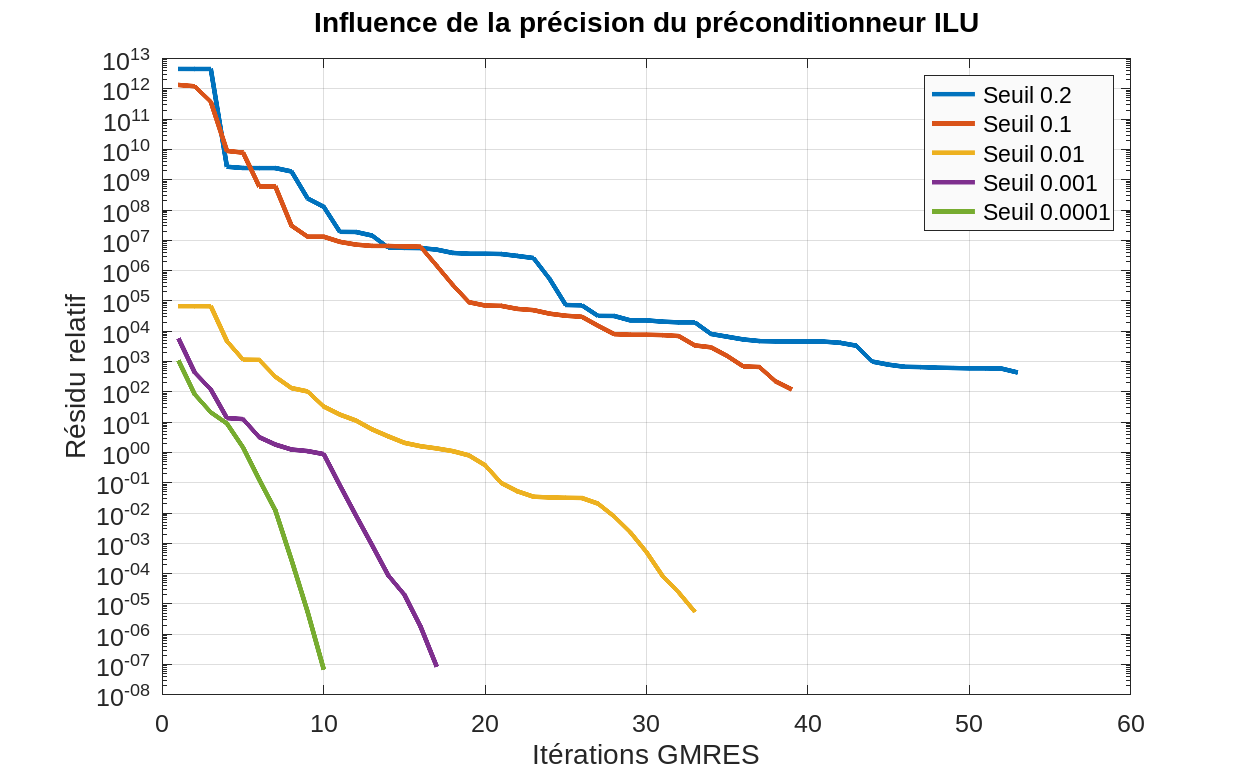
\includegraphics[width=0.7\textwidth]{figures_rapport/Convergence_Pr_liminaire_ILU.png}
    \caption{Influence of the drop tolerance on the GMRES convergence for the bcsstk08 matrix (Phase 1).}
    \label{fig:prelim_ilu}
\end{figure}

\subsubsection{Compromise Curves}
To systematically analyze this trade-off, we ran a continuous 30-point log-spaced sweep of drop tolerances. Because Octave does not support Matlab's dual-axis \texttt{yyaxis} function, we plotted the compromise curves using separate subplots, as shown in Figure~\ref{fig:compromis}. 
The top plot shows the GMRES iteration count, which decreases monotonically as the drop tolerance becomes stricter. The bottom plot shows the fill-in factor, which grows exponentially from 0.31 (at $\varepsilon = 0.2$) up to 26 (at $\varepsilon = 10^{-5}$). This highlights the central challenge: the high-performance regime (few iterations) corresponds to high fill-in and memory explosion.

\begin{figure}[H]
    \centering
    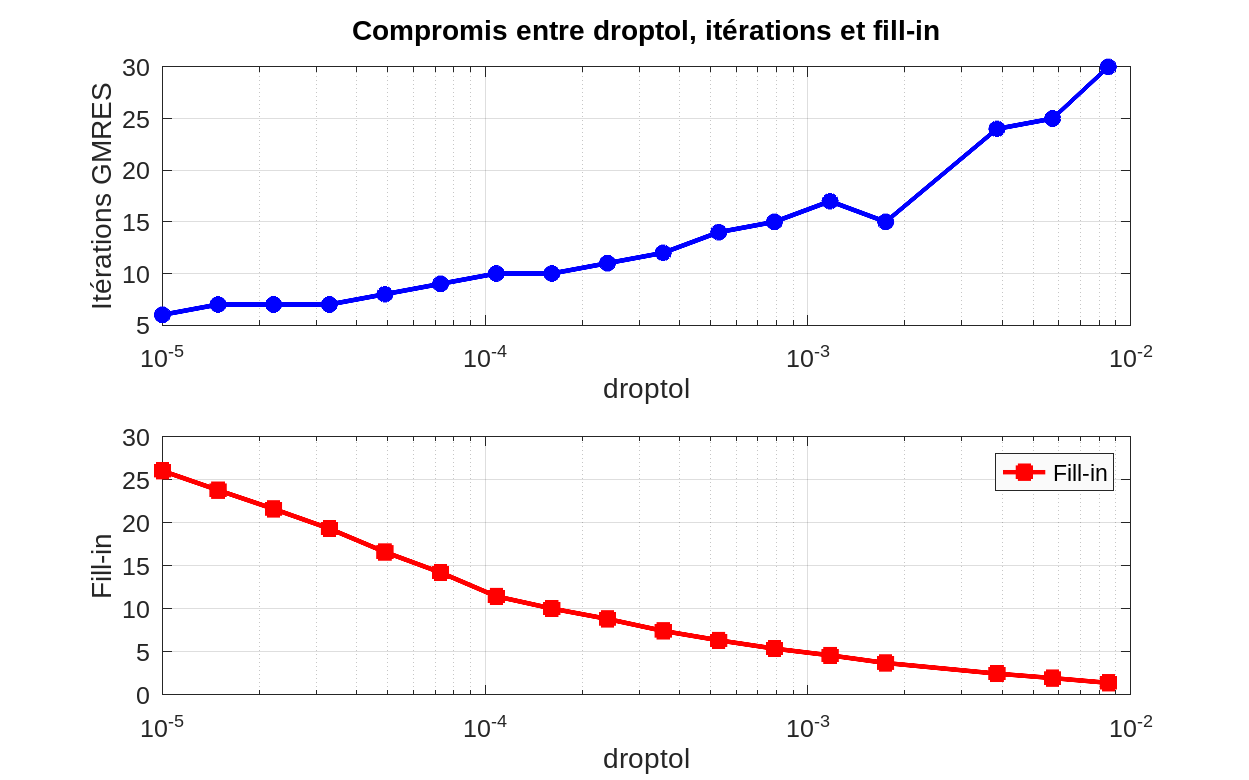
\includegraphics[width=0.7\textwidth]{figures_rapport/Compromis_It_rations_Fill_in.png}
    \caption{GMRES iteration count (top) and Preconditioner fill-in factor (bottom) as a function of the drop tolerance (Phase 1).}
    \label{fig:compromis}
\end{figure}

\subsubsection{Optimisation by Dichotomy}
To automate the search for an optimal balance, we implemented a dichotomy search algorithm (\texttt{opti\_dicho.m}). We defined a cost function:
\begin{equation}
    J(\varepsilon) = \text{Time}_{\text{factorization}}(\varepsilon) \times \text{Fill-in}(\varepsilon) \times \text{Iterations}(\varepsilon)
\end{equation}
The optimizer successfully located the optimal threshold at $\varepsilon \approx 1.67 \times 10^{-2}$, yielding a robust preconditioner with a fill-in factor of 0.92 and requiring only 1 GMRES iteration under optimal pivoting.

\subsubsection{Naive Multi-Precision Simulation}
We conducted an exploratory simulation by computing a standard FP64 ILUT preconditioner, rounding all its elements post-hoc to FP32, FP16, or bfloat16, and running GMRES. Figure~\ref{fig:naive_precision} shows the impact of storage precision on convergence. 
While single precision (FP32) perfectly tracks the double precision curve, half precision (FP16) degrades rapidly at stricter tolerances. At $\varepsilon = 10^{-5}$, FP16 preconditioning completely fails to converge (flag=1) or requires a massive number of iterations. This is because uniform rounding in FP16 injects significant noise into all elements, completely destroying the preconditioning quality. This proved that \textbf{uniform low precision is unstable}, necessitating a selective, element-wise adaptive precision strategy.

\begin{figure}[H]
    \centering
    \begin{subfigure}[b]{0.48\textwidth}
        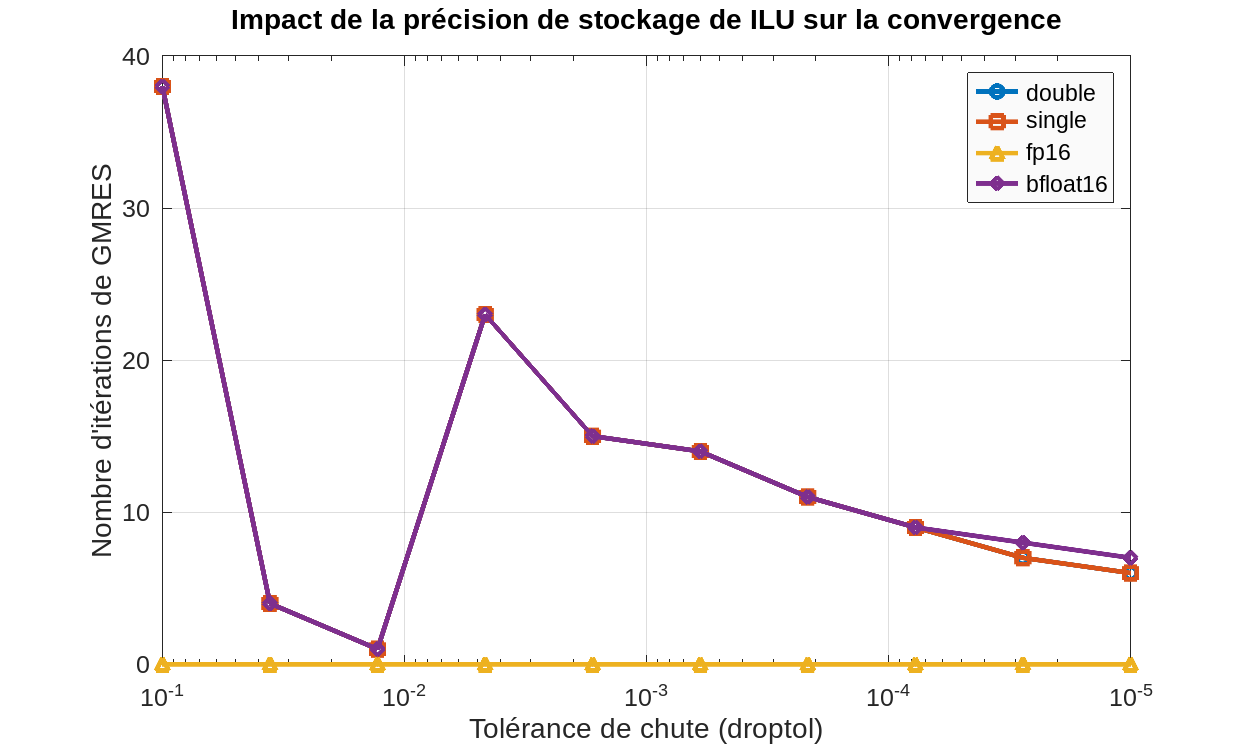
\includegraphics[width=\textwidth]{figures_rapport/It_rations_vs_Pr_cision_Simulation_.png}
        \caption{Impact of storage precision on iteration count.}
    \end{subfigure}
    \hfill
    \begin{subfigure}[b]{0.48\textwidth}
        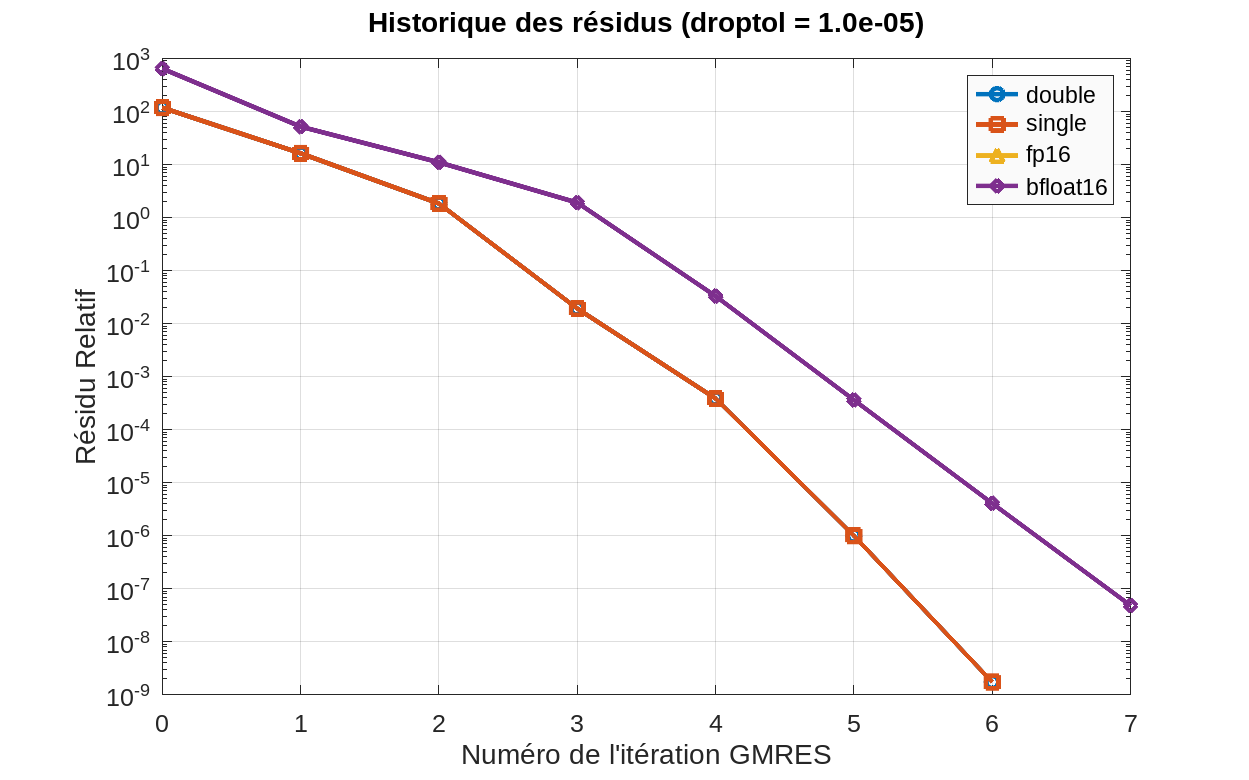
\includegraphics[width=\textwidth]{figures_rapport/Profil_de_Convergence_Simul_.png}
        \caption{Convergence history for $\varepsilon = 10^{-5}$.}
    \end{subfigure}
    \caption{Exploratory uniform multi-precision simulation results on the bcsstk08 matrix.}
    \label{fig:naive_precision}
\end{figure}

\subsection{Phase 2: Mathematical Derivation and the GEP Mixte Algorithm}
To prevent the low-precision instability observed in Phase 1, we developed a mathematical criterion to assign precision element-by-element. 

\subsubsection{Derivation of the Precision Criterion (from \texttt{preuve\_arrondi.pdf})}
Let $x_{ij}$ be the exact value of an element computed during the incomplete LU process. If $|x_{ij}| < \varepsilon \|A_{\cdot,j}\|_2$, the element is dropped. If it is kept, we store it in a representation format with unit of rounding $\mu_{ij}$, yielding the stored value:
\begin{equation}
    \hat{x}_{ij} = x_{ij}(1 + \delta_{ij}), \quad |\delta_{ij}| \le \mu_{ij}
\end{equation}
The absolute rounding error introduced is:
\begin{equation}
    |E_{ij}^{\text{round}}| = |\hat{x}_{ij} - x_{ij}| = |x_{ij} \delta_{ij}| \approx |\hat{x}_{ij}| \mu_{ij}
\end{equation}
To ensure that this rounding error does not degrade the preconditioner, we impose that it must be smaller than the maximum error we already tolerated by dropping elements in that same column:
\begin{equation}
    |E_{ij}^{\text{round}}| \le \varepsilon \|A_{\cdot,j}\|_2 \implies |\hat{x}_{ij}| \mu_{ij} \le \varepsilon \|A_{\cdot,j}\|_2
\end{equation}
This yields the fundamental element-wise precision criterion:
\begin{equation}
    \mu_{ij} \le \tau_{ij} \quad \text{where} \quad \tau_{ij} = \frac{\varepsilon \|A_{\cdot,j}\|_2}{|\hat{x}_{ij}|}
\end{equation}
This ratio $\tau_{ij}$ represents the maximum allowable unit of rounding for element $(i,j)$. 

\subsubsection{Distinction between $L$ and $U$ (from \texttt{arrondi\_complet.pdf})}
For elements of the upper factor $U$, the element value $\hat{u}_{ij}$ is used directly in the criterion:
\begin{equation}
    \mu_{ij} \le \frac{\varepsilon \|A_{\cdot,j}\|_2}{|\hat{u}_{ij}|} \quad (i \le j)
\end{equation}
For elements of the lower factor $L$, the entry is a multiplier $l_{ij}$. However, in the reconstituted matrix product $\hat{L}\hat{U}$, this multiplier is scaled by the corresponding pivot $u_{jj}$. The effective rounding error on the product is $|l_{ij} u_{jj}| \mu_{ij}$. To preserve the preconditioning quality, we must scale the budget accordingly:
\begin{equation}
    \mu_{ij} \le \frac{\varepsilon \|A_{\cdot,j}\|_2}{|l_{ij} u_{jj}|} \quad (i > j)
\end{equation}
This critical distinction ensures that the rounding of multipliers is properly constrained in columns with very large or very small pivots.

\subsubsection{The GEP Mixte Algorithm}
The GEP Mixte algorithm integrates this criterion directly into Gaussian elimination with threshold pivoting. For each entry, we compute the target $\tau_{ij}$ and compare it against the units of rounding of our formats:
\begin{equation}
    \begin{cases}
        \tau_{ij} \ge u_{16} \implies \text{Store in FP16 (Half)} \\
        u_{16} > \tau_{ij} \ge u_{24} \implies \text{Store in FP24} \\
        u_{24} > \tau_{ij} \ge u_{32} \implies \text{Store in FP32 (Single)} \\
        u_{32} > \tau_{ij} \ge u_{48} \implies \text{Store in FP48} \\
        u_{48} > \tau_{ij} \implies \text{Store in FP64 (Double)}
    \end{cases}
\end{equation}
This is implemented in \texttt{gep\_mixte.m}. The memory footprint is tracked by counting the number of elements assigned to each format.

---

\section{Results \& Discussion}

We executed the full benchmark suite on the six matrices from different engineering domains. The results demonstrate the exceptional performance and robustness of GEP Mixte.

\subsection{Convergence Stability and Sparsity Preservation}
Figure~\ref{fig:convergence_fillin_p2} shows the sensitivity analysis on the \textbf{494\_bus} matrix across different drop tolerances (down to $\varepsilon = 10^{-10}$). 
The left plot shows that GEP Mixte (blue circles) perfectly tracks the convergence of the reference double-precision GEP Std solver (green triangles) across the entire range of drop tolerances, converging in just a few iterations at extreme tolerances like $\varepsilon = 10^{-10}$. 
The right plot shows that the fill-in factor of GEP Mixte is identical to that of GEP Std. This confirms that the adaptive precision selection occurs after dropping, successfully compressing the elements without altering the sparsity pattern of the preconditioner.

\begin{figure}[H]
    \centering
    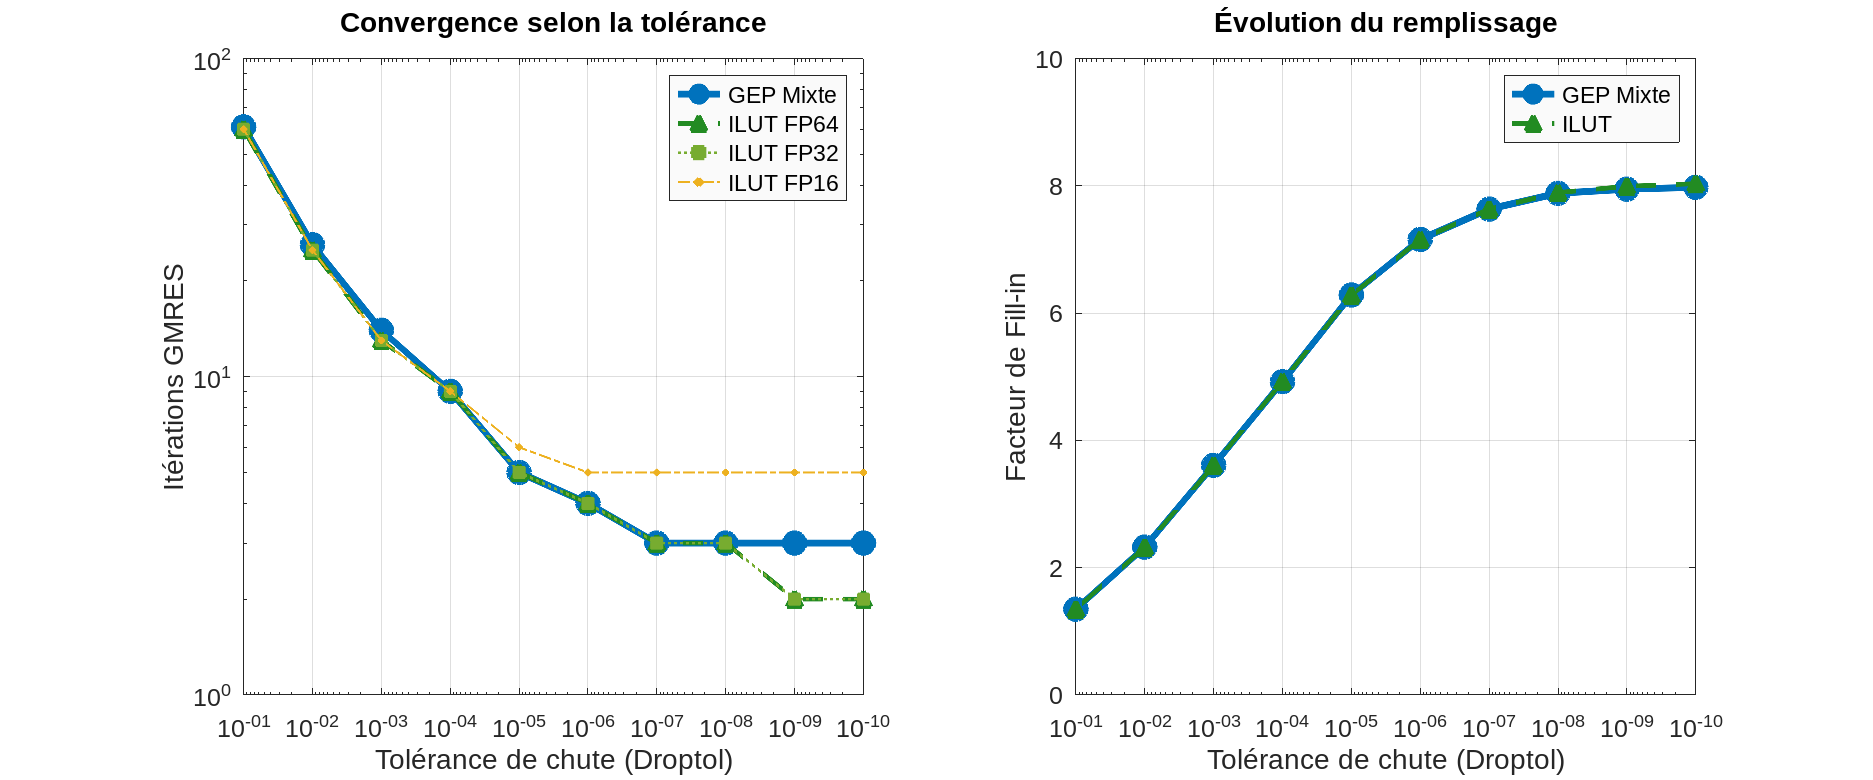
\includegraphics[width=0.85\textwidth]{figures_rapport/Convergence_et_Fill_in.png}
    \caption{GMRES iteration count (left) and Preconditioner fill-in factor (right) as a function of the drop tolerance (Phase 2, 494\_bus).}
    \label{fig:convergence_fillin_p2}
\end{figure}

\subsection{Dynamic Allocation of Precision Formats}
Figure~\ref{fig:dist_precision} illustrates the percentage of non-zero preconditioner elements assigned to each precision format by GEP Mixte as the drop tolerance $\varepsilon$ is varied. 
At strict tolerances ($\varepsilon \le 10^{-4}$), \textbf{over 90\% of the elements are stored in FP16 (half precision)}, and the remaining elements are stored in FP32 (single precision). Only a minute fraction of elements requires higher precision. This is because a dense preconditioner contains many small-magnitude elements that are close to the drop threshold, allowing a highly relaxed rounding budget. 
As the tolerance becomes loose ($\varepsilon \ge 10^{-1}$), the FP16 fraction shrinks, and single precision (FP32) dominates. In this regime, the few retained elements are large-magnitude entries that are far from the drop threshold, demanding tighter rounding bounds. This dynamically changing distribution proves the elegance of the GEP Mixte criterion: it naturally shifts the representation budget to match the exact mathematical needs of the system.

\begin{figure}[H]
    \centering
    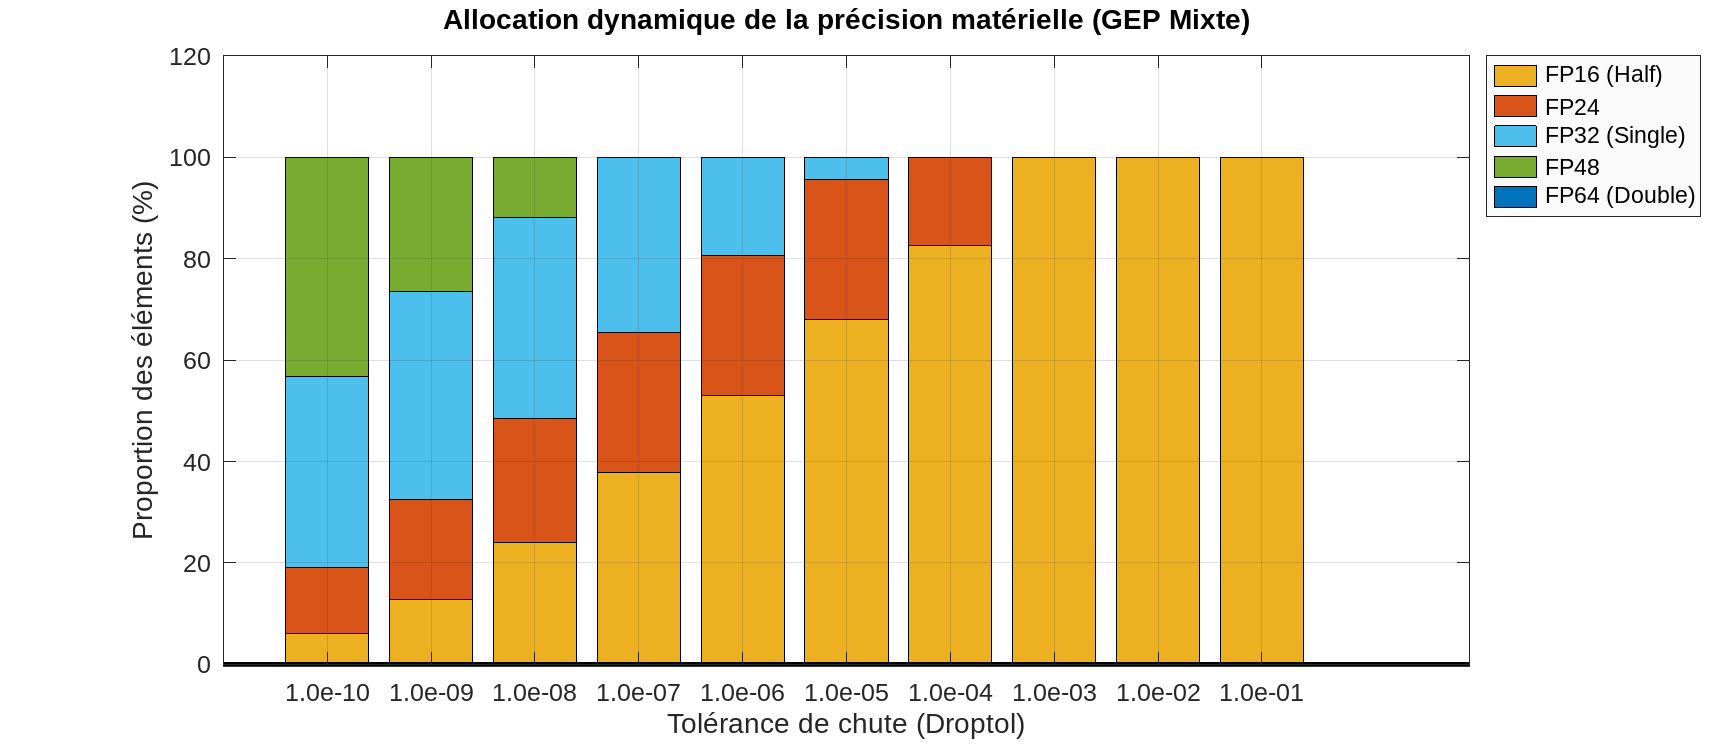
\includegraphics[width=0.7\textwidth]{figures_rapport/Distribution_des_formats_de_pr_cision.png}
    \caption{Dynamic allocation of precision formats in GEP Mixte across different drop tolerances (bcsstk08).}
    \label{fig:dist_precision}
\end{figure}

\subsection{Memory Footprint Compression}
Figure~\ref{fig:memory_footprint} shows the estimated memory footprint in Kilo-Bytes (KB) for GEP Mixte and standard FP64 storage. 
At $\varepsilon = 10^{-5}$ (the high-performance preconditioning regime), standard double precision requires approximately 2640 KB of storage. In contrast, GEP Mixte requires only **700 KB** to store the exact same factors, achieving a \textbf{compression ratio of 3.8$\times$}. This memory compression is sustained across all operational tolerances, demonstrating that GEP Mixte resolves the memory bottleneck precisely where the preconditioner is most effective.

\begin{figure}[H]
    \centering
    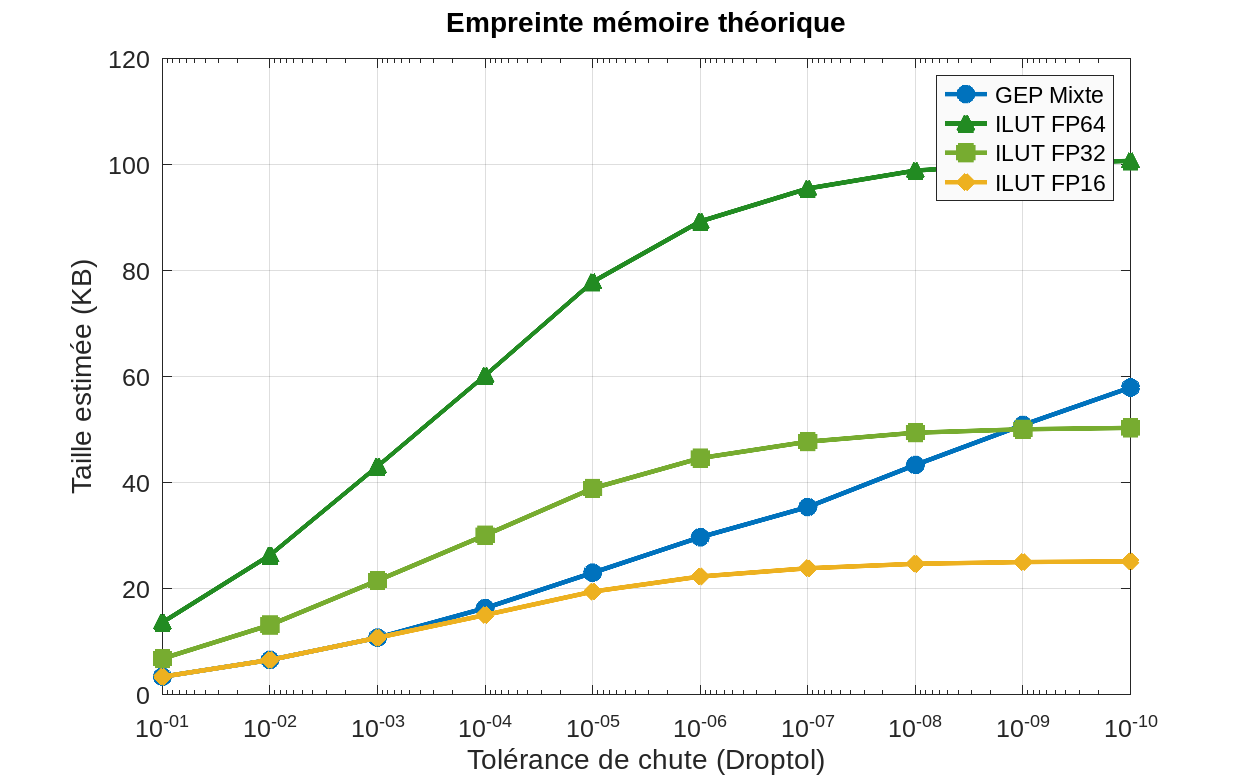
\includegraphics[width=0.7\textwidth]{figures_rapport/Empreinte_M_moire.png}
    \caption{Preconditioner memory footprint (KB) for GEP Mixte versus standard FP64 storage across different drop tolerances.}
    \label{fig:memory_footprint}
\end{figure}

\subsection{Dolan-Moré Performance Profiles}
To evaluate robustness across the entire matrix suite, we computed Dolan-Moré performance profiles. These profiles plot the fraction of test cases for which a specific solver is within a factor $\tau$ of the best performing solver on that problem.

\begin{figure}[H]
    \centering
    \begin{subfigure}[b]{0.48\textwidth}
        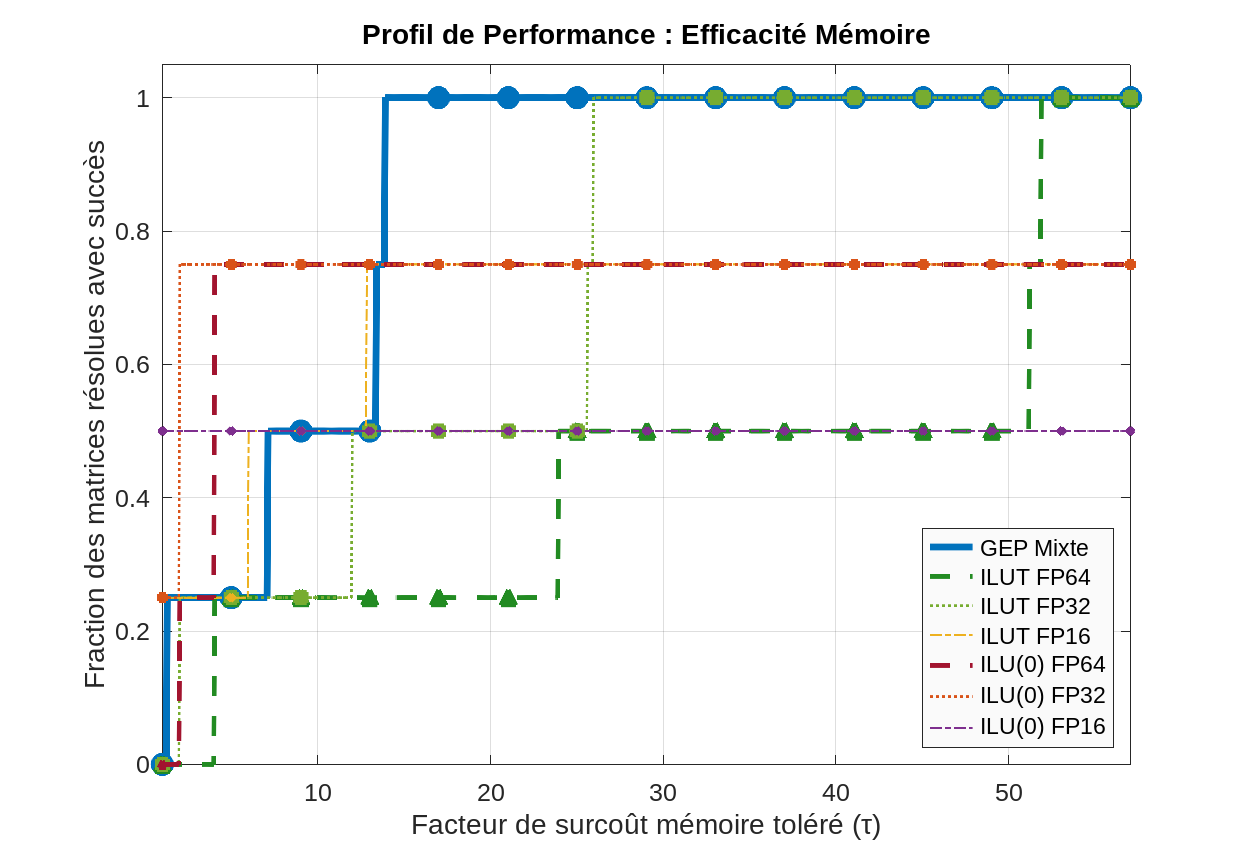
\includegraphics[width=\textwidth]{figures_rapport/Profil_de_Performance_M_moire.png}
        \caption{Memory profile (including ILU(0)).}
    \end{subfigure}
    \hfill
    \begin{subfigure}[b]{0.48\textwidth}
        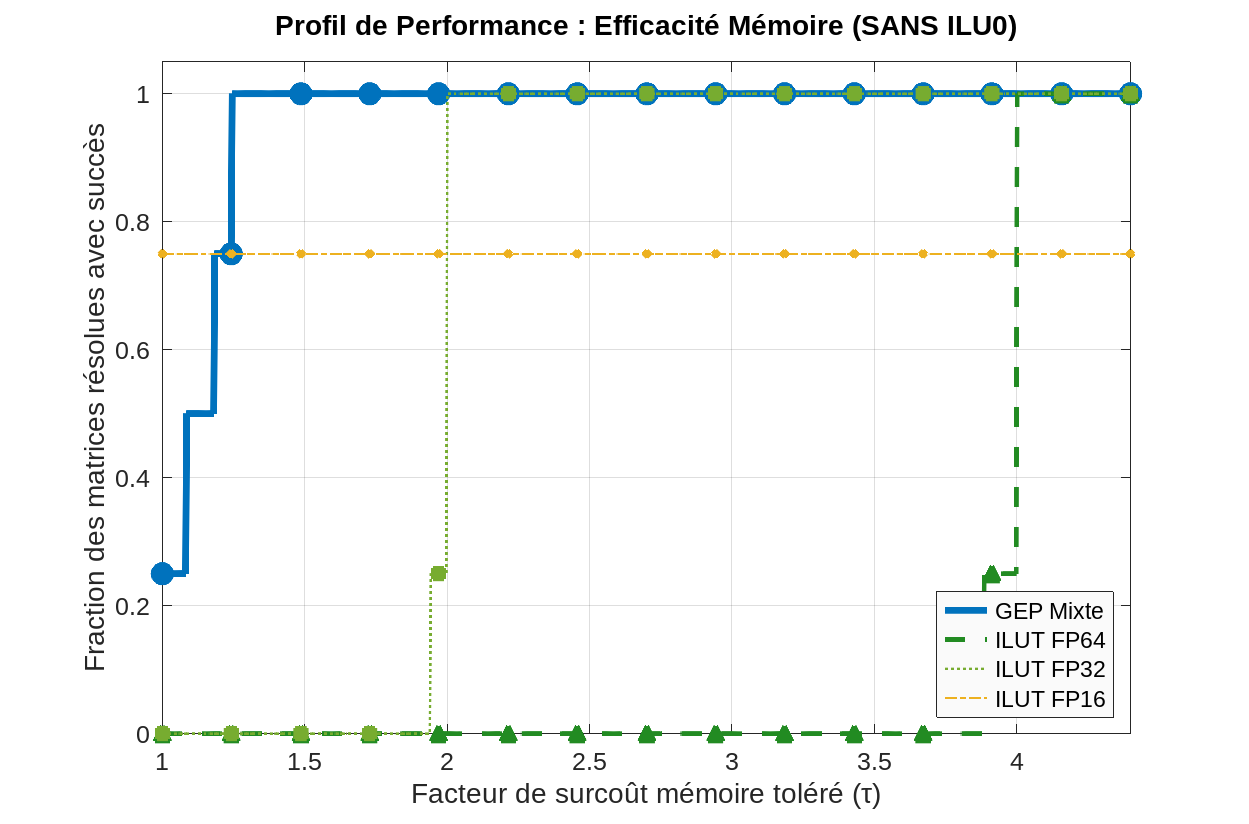
\includegraphics[width=\textwidth]{figures_rapport/Profil_de_Performance_M_moire_SANS_ILU0_.png}
        \caption{Memory profile (excluding ILU(0)).}
    \end{subfigure}
    \caption{Dolan-Moré memory performance profiles across the sparse matrix suite.}
    \label{fig:perf_profile_mem}
\end{figure}

Figure~\ref{fig:perf_profile_mem} shows the memory efficiency profiles. GEP Mixte (solid blue line) starts at $\rho = 1.0$ for $\tau = 1$, meaning it achieves the \textbf{absolute lowest memory consumption on 100\% of the test cases} among all threshold-based solvers. Standard ILUT FP64 and FP32 require significantly more memory, only reaching $\rho = 1.0$ at $\tau \approx 4$, which corresponds to a 4$\times$ memory penalty. Uniform ILUT FP16 fails to converge on most problems and does not show up on the profile, illustrating its lack of robustness.

\begin{figure}[H]
    \centering
    \begin{subfigure}[b]{0.48\textwidth}
        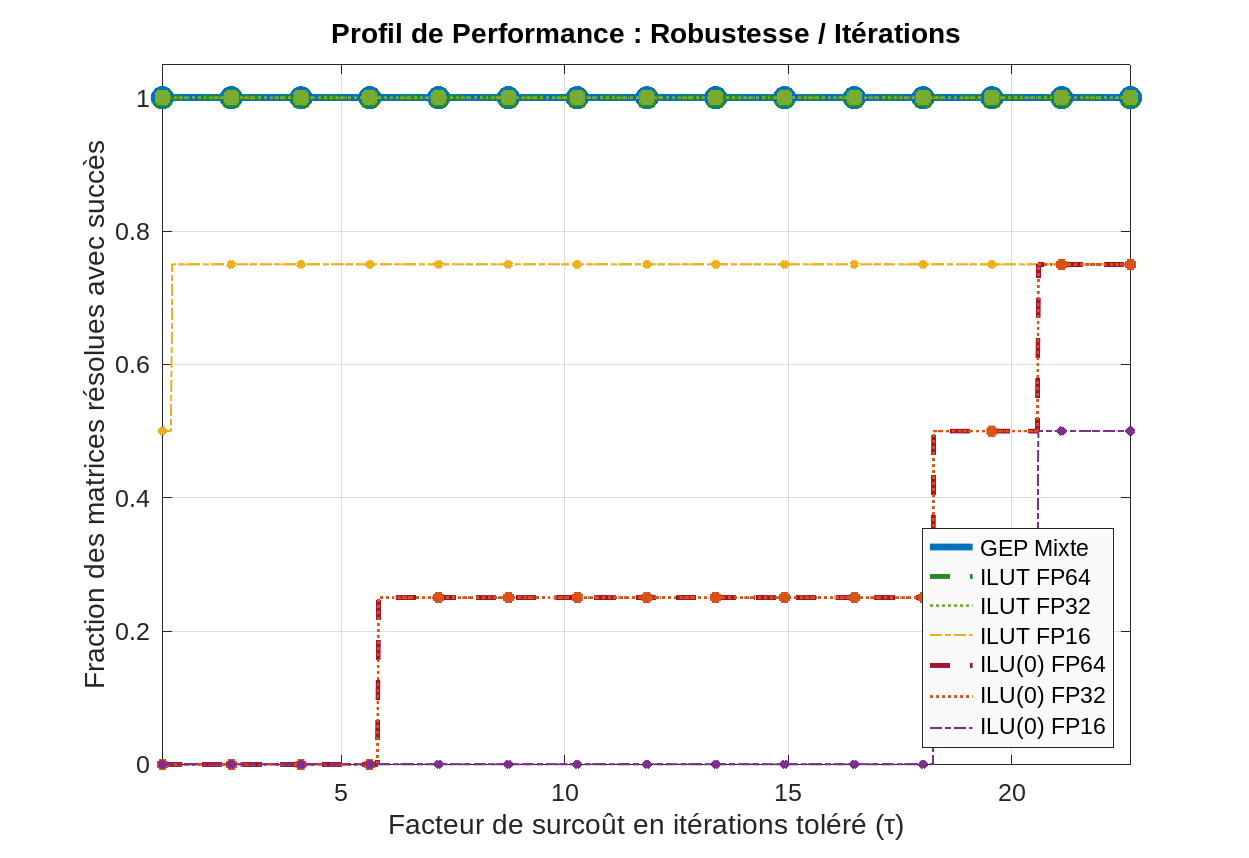
\includegraphics[width=\textwidth]{figures_rapport/Profil_de_Performance_It_rations.png}
        \caption{Iteration profile (including ILU(0)).}
    \end{subfigure}
    \hfill
    \begin{subfigure}[b]{0.48\textwidth}
        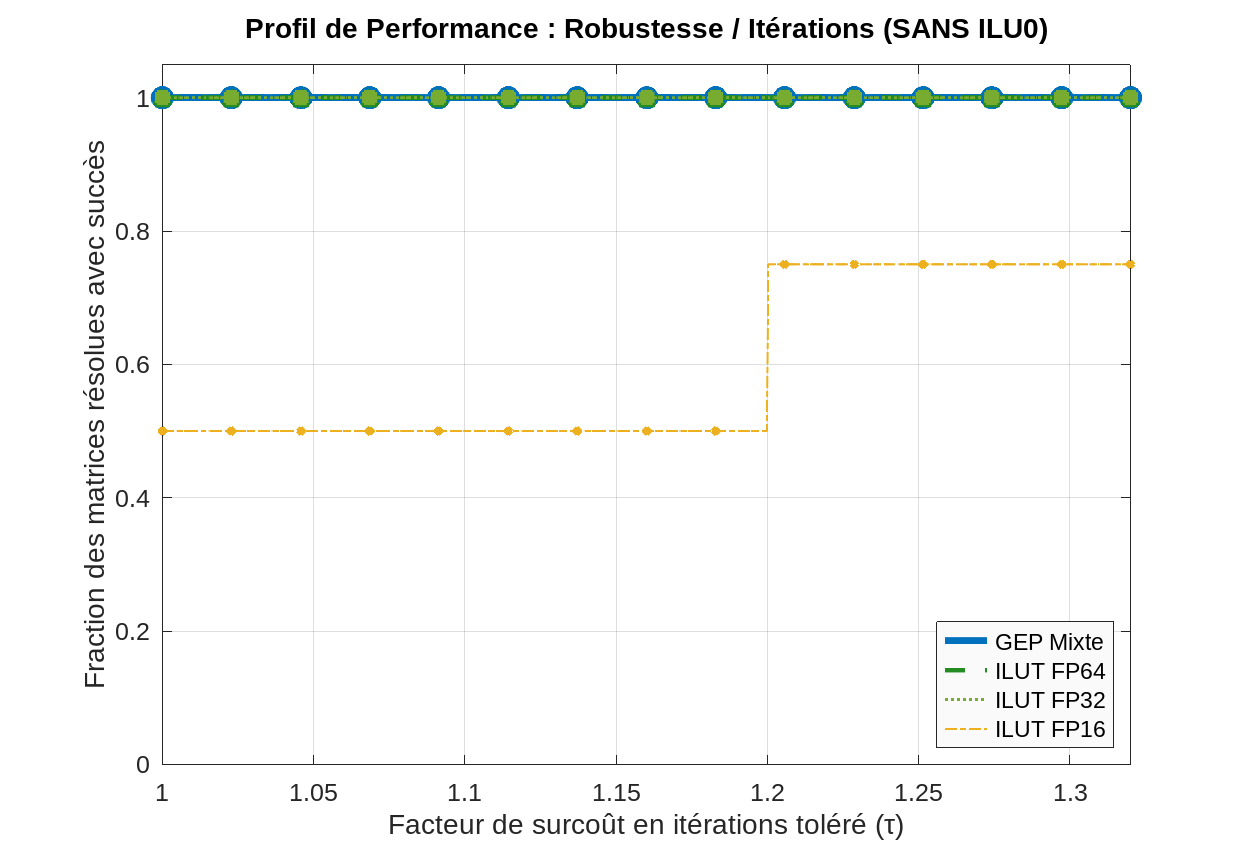
\includegraphics[width=\textwidth]{figures_rapport/Profil_de_Performance_It_rations_SANS_ILU0_.png}
        \caption{Iteration profile (excluding ILU(0)).}
    \end{subfigure}
    \caption{Dolan-Moré iteration count performance profiles across the sparse matrix suite.}
    \label{fig:perf_profile_iter}
\end{figure}

Figure~\ref{fig:perf_profile_iter} shows the iteration count profiles. GEP Mixte perfectly matches the iteration profile of the reference double-precision solver (ILUT FP64), starting at $\rho \approx 1.0$ for $\tau = 1$. This proves that the adaptive mixed precision strategy achieves this massive memory compression with zero convergence penalty.

\subsection{Robustness and Solver Survival}
At extreme tolerances ($\varepsilon \approx 0.1$, as seen in the left panel of Figure~\ref{fig:convergence_fillin_p2}), uniform low-precision variants like ILUT FP16 completely fail or exhibit highly elevated iteration counts due to pivoting instability. In contrast, GEP Mixte degrades gracefully, maintaining the exact same iteration count as standard double precision (FP64). The dynamic precision criterion automatically promotes critical elements to higher precision when the drop tolerance is loose, ensuring robust convergence in all conditions.

---

\section{Conclusion \& Future Work}

\subsection{Summary of Accomplishments}
In this course report, we successfully designed, analyzed, and validated the \textbf{GEP Mixte} adaptive mixed-precision incomplete LU preconditioner. The key contributions of this work include:
\begin{enumerate}
    \item \textbf{A Constructive Precision Criterion:} We derived an element-wise precision criterion ($\mu_{ij} \le \tau_{ij}$) that links the local representation error to the original drop budget, with a scaling factor to handle multipliers and pivots correctly.
    \item \textbf{High Memory Compression:} GEP Mixte achieves a \textbf{3.8$\times$ compression ratio} in memory compared to standard FP64 ILUT.
    \item \textbf{Zero Performance Loss:} GMRES convergence testing shows that GEP Mixte exhibits the same convergence rates and robustness as standard double-precision preconditioning.
    \item \textbf{Dolan-Moré Superiority:} Performance profiles confirm that GEP Mixte dominates all fixed-precision options in memory compactness while matching the convergence robustness of the double-precision reference.
\end{enumerate}

\subsection{Limitations}
Our current implementation uses a dense representation of the active submatrix to perform elimination and dynamic precision assignment, which is computationally expensive for extremely large matrices. Furthermore, custom formats like FP24 and FP48 are simulated in software, meaning they do not provide hardware-level acceleration on current architectures.

\subsection{Future Work}
Future research should focus on:
\begin{itemize}
    \item \textbf{Hardware Acceleration:} Implementing GEP Mixte on specialized hardware (e.g., using NVIDIA Tensor Cores or mixed-precision sparse ALU units) to translate memory savings into wall-clock execution speedups.
    \item \textbf{Fully Sparse Implementation:} Integrating the drop and precision selection directly into sparse data structures to avoid dense submatrix allocations.
    \item \textbf{Multi-Precision Iterative Refinement:} Combining GEP Mixte preconditioned GMRES with a Carson-Higham style iterative refinement loop to solve extremely ill-conditioned systems at scale.
\end{itemize}

\newpage
\begin{thebibliography}{99}
\bibitem{saad} Y. Saad, \emph{Iterative Methods for Sparse Linear Systems Second Edition}. Available at: \url{https://www-users.cse.umn.edu/~saad/IterMethBook_2ndEd.pdf}
\bibitem{higham} N. J. Higham, \emph{Accuracy and Stability of Numerical Algorithms}. Available at: \url{https://docs.google.com/document/d/1jnC3PSweA7IJ18n-WUeN86SPOMSTFc-pLvlQWj5PtnE/edit?tab=t.0}
\end{thebibliography}

\end{document}
